% Generated 2021-08-25 18:02:25 +0530
\subsection{RawMaterial} \label{sec:RawMaterial}


This section provides the semantic information for the \block{RawMaterial} model.

\begin{figure}[ht]
  \centering
    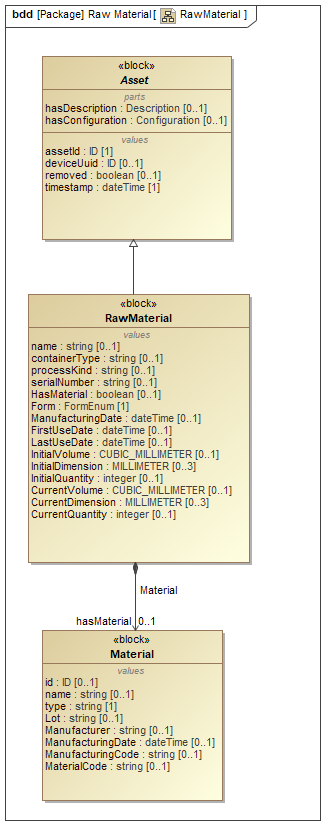
\includegraphics[width=1.0\textwidth]{figures/RawMaterial.png}
  \caption{RawMaterial Diagram}
  \label{fig:RawMaterial Diagram}
\end{figure}

\FloatBarrier


Note: See \sect{RawMaterial Schema Diagrams} for XML schema.


\subsubsection{RawMaterial}




\block{RawMaterial} is an \block{Asset} that represents \gls{raw material}.


\paragraph{Attributes of RawMaterial}\mbox{}
\label{sec:Attributes of RawMaterial}

\tbl{Attributes of RawMaterial} lists the attributes of \texttt{RawMaterial}.

\begin{table}[ht]
\centering 
  \caption{Attributes of RawMaterial}
  \label{table:Attributes of RawMaterial}
\tabulinesep=3pt
\begin{tabu} to 6in {|l|l|l|} \everyrow{\hline}
\hline
\rowfont\bfseries {Attribute} & {Type} & {Multiplicity} \\
\tabucline[1.5pt]{}

\property{name}[RawMaterial] & \texttt{string} & 0..1 \\
\property{containerType}[RawMaterial] & \texttt{string} & 0..1 \\
\property{processKind}[RawMaterial] & \texttt{string} & 0..1 \\
\property{serialNumber}[RawMaterial] & \texttt{string} & 0..1 \\
\end{tabu}
\end{table}
\FloatBarrier

Descriptions for attributes of \block{RawMaterial}:

\begin{itemize}

\item \property{name}[RawMaterial] \newline The \gls{raw material} name.

Examples: \texttt{Container1} and \texttt{AcrylicContainer}.

\item \property{containerType}[RawMaterial] \newline The type of container holding the \gls{raw material}. 

Examples: \texttt{Pallet}, \texttt{Canister}, \texttt{Cartridge}, \texttt{Tank}, \texttt{Bin}, \texttt{Roll}, and \texttt{Spool}.

\item \property{processKind}[RawMaterial] \newline The ISO process type supported by this \gls{raw material}. 

Examples include: \texttt{VAT\textunderscore POLYMERIZATION}, \texttt{BINDER\textunderscore JETTING}, \texttt{MATERIAL\textunderscore EXTRUSION}, \texttt{MATERIAL\textunderscore JETTING}, \texttt{SHEET\textunderscore LAMINATION}, \texttt{POWDER\textunderscore BED\textunderscore FUSION} and \texttt{DIRECTED\textunderscore ENERGY\textunderscore DEPOSITION}.

\item \property{serialNumber}[RawMaterial] \newline The serial number of the \gls{raw material}.
\end{itemize}


\paragraph{Elements of RawMaterial}\mbox{}
\label{sec:Elements of RawMaterial}

\tbl{Elements of RawMaterial} lists the elements of \texttt{RawMaterial}.

\begin{table}[ht]
\centering 
  \caption{Elements of RawMaterial}
  \label{table:Elements of RawMaterial}
\tabulinesep=3pt
\begin{tabu} to 6in {|l|l|} \everyrow{\hline}
\hline
\rowfont\bfseries {Element} & {Multiplicity} \\
\tabucline[1.5pt]{}
\texttt{HasMaterial} & 0..1 \\
\texttt{Material} & 0..1 \\
\texttt{Form} & 1 \\
\texttt{ManufacturingDate} & 0..1 \\
\texttt{FirstUseDate} & 0..1 \\
\texttt{LastUseDate} & 0..1 \\
\texttt{InitialVolume} & 0..1 \\
\texttt{InitialDimension} & 0..1 \\
\texttt{InitialQuantity} & 0..1 \\
\texttt{CurrentVolume} & 0..1 \\
\texttt{CurrentDimension} & 0..1 \\
\texttt{CurrentQuantity} & 0..1 \\
\end{tabu}
\end{table}
\FloatBarrier


Descriptions for elements of \block{RawMaterial}:

\begin{itemize}

\item \block{HasMaterial} \newline \block{Material} has existing usable volume.

The value of \block{HasMaterial} \MUST be \texttt{boolean}.

\item \block{Material} \newline Material used as the \block{RawMaterial}

\item \block{Form} \newline The form of the \gls{raw material}.

\texttt{FormEnum} Enumeration:

\begin{itemize}
\item \texttt{BAR} \newline  
\item \texttt{SHEET} \newline  
\item \texttt{BLOCK} \newline  
\item \texttt{CASTING} \newline  
\item \texttt{POWDER} \newline  
\item \texttt{LIQUID} \newline  
\item \texttt{GEL} \newline  
\item \texttt{FILAMENT} \newline  
\item \texttt{GAS} \newline  
\end{itemize}


\item \block{ManufacturingDate} \newline The date the \gls{raw material} was created.

The value of \block{ManufacturingDate} \MUST be \texttt{dateTime}.

\item \block{FirstUseDate} \newline The date \gls{raw material} was first used.

The value of \block{FirstUseDate} \MUST be \texttt{dateTime}.

\item \block{LastUseDate} \newline The date \gls{raw material} was last used.

The value of \block{LastUseDate} \MUST be \texttt{dateTime}.

\item \block{InitialVolume} \newline The amount of material initially placed in \gls{raw material} when manufactured.

The value \textbf{MUST} be reported in \texttt{MILLIMETER\textunderscore 3D}.

The value of \block{InitialVolume} \MUST be \texttt{float}.

\item \block{InitialDimension} \newline The dimension of material initially placed in \gls{raw material} when manufactured.

The value \textbf{MUST} be reported in \texttt{MILLIMETER\textunderscore 3D}.

The value of \block{InitialDimension} \MUST be \texttt{float}.

\item \block{InitialQuantity} \newline The quantity of material initially placed in \gls{raw material} when manufactured.

The value of \block{InitialQuantity} \MUST be \texttt{integer}.

\item \block{CurrentVolume} \newline  The amount of material currently in \gls{raw material}.

The value \textbf{MUST} be reported in \texttt{MILLIMETER\textunderscore 3D}.

The value of \block{CurrentVolume} \MUST be \texttt{float}.

\item \block{CurrentDimension} \newline The dimension of material currently in \gls{raw material}.

The value \textbf{MUST} be reported in \texttt{MILLIMETER\textunderscore 3D}.

The value of \block{CurrentDimension} \MUST be \texttt{float}.

\item \block{CurrentQuantity} \newline The quantity of material currently in \gls{raw material}.

The value of \block{CurrentQuantity} \MUST be \texttt{integer}.
\end{itemize}



\subsubsection{Material}
\label{sec:Material}



Material used as the \block{RawMaterial}


\paragraph{Attributes of Material}\mbox{}
\label{sec:Attributes of Material}

\tbl{Attributes of Material} lists the attributes of \texttt{Material}.

\begin{table}[ht]
\centering 
  \caption{Attributes of Material}
  \label{table:Attributes of Material}
\tabulinesep=3pt
\begin{tabu} to 6in {|l|l|l|} \everyrow{\hline}
\hline
\rowfont\bfseries {Attribute} & {Type} & {Multiplicity} \\
\tabucline[1.5pt]{}

\property{id}[Material] & \texttt{ID} & 0..1 \\
\property{name}[Material] & \texttt{string} & 0..1 \\
\property{type}[Material] & \texttt{string} & 1 \\
\end{tabu}
\end{table}
\FloatBarrier

Descriptions for attributes of \block{Material}:

\begin{itemize}

\item \property{id}[Material] \newline The unique identifier for the material.

\item \property{name}[Material] \newline The name of the material. Examples: \texttt{ULTM9085}, \texttt{ABS}, \texttt{4140}.

\item \property{type}[Material] \newline The type of material. Examples: \texttt{Metal}, \texttt{Polymer}, \texttt{Wood}, \texttt{4140}, \texttt{Recycled}, \texttt{Prestine} and \texttt{Used}.
\end{itemize}


\paragraph{Elements of Material}\mbox{}
\label{sec:Elements of Material}

\tbl{Elements of Material} lists the elements of \texttt{Material}.

\begin{table}[ht]
\centering 
  \caption{Elements of Material}
  \label{table:Elements of Material}
\tabulinesep=3pt
\begin{tabu} to 6in {|l|l|} \everyrow{\hline}
\hline
\rowfont\bfseries {Element} & {Multiplicity} \\
\tabucline[1.5pt]{}
\texttt{Lot} & 0..1 \\
\texttt{Manufacturer} & 0..1 \\
\texttt{ManufacturingDate} & 0..1 \\
\texttt{ManufacturingCode} & 0..1 \\
\texttt{MaterialCode} & 0..1 \\
\end{tabu}
\end{table}
\FloatBarrier


Descriptions for elements of \block{Material}:

\begin{itemize}

\item \block{Lot} \newline The manufacturer's lot code of the material.

The value of \block{Lot} \MUST be \texttt{string}.

\item \block{Manufacturer} \newline The name of the material manufacturer.

The value of \block{Manufacturer} \MUST be \texttt{string}.

\item \block{ManufacturingDate} \newline The manufacturing date of the material from the material manufacturer.

The value of \block{ManufacturingDate} \MUST be \texttt{dateTime}.

\item \block{ManufacturingCode} \newline The lot code of the raw feed stock for the material, from the feed stock manufacturer.

The value of \block{ManufacturingCode} \MUST be \texttt{string}.

\item \block{MaterialCode} \newline The \gls{ASTM} standard code that the material complies with.

The value of \block{MaterialCode} \MUST be \texttt{string}.
\end{itemize}


